\documentclass{article}
\usepackage{amsmath}
\usepackage{graphicx}
\usepackage{listings}
\usepackage{fullpage}
\usepackage{courier}
\usepackage{float}  % Ensures figure placement

\lstset{
  basicstyle=\ttfamily\footnotesize,
  breaklines=true,
  frame=single,
}

\begin{document}

\section*{A5}

\subsection*{(a)}

Many features in the dataset are influenced by historical policy decisions in the U.S., as laws, government funding, and policy priorities shape economic, law enforcement, and urban development outcomes. Below are three examples of such features:

\begin{itemize}
    \item \textbf{Per Capita Income}: 
    Government policies such as tax regulations, minimum wage laws, social security benefits, and job creation programs directly influence income distribution across communities. Additionally, differences in \textit{state income tax} policies can lead to significant variations in per capita income, as states with lower taxes may attract higher-income residents while others use tax revenues for social welfare programs.
    
    \item \textbf{Public Transportation Usage}: 
    The availability and usage of public transit systems are heavily dependent on government infrastructure investments, zoning laws, and urban planning policies. Cities with significant public transit funding tend to have higher ridership, whereas communities with lower investments force residents to rely on personal vehicles, affecting commuting patterns and economic mobility.
    
    \item \textbf{Police Budget Allocation}: 
    Law enforcement funding is determined by local and federal budget allocations, city council decisions, and crime prevention policies. Some municipalities prioritize increased policing with higher budgets, while others may divert resources toward community programs, education, or social services, leading to variation in police funding across different areas.
\end{itemize}

These examples illustrate how government decisions and policies shape the data in ways that are not purely demographic or economic but instead reflect historical and political choices.

\subsection*{(b)}

Some features in the dataset might be found to have nonzero weights in the model, suggesting a correlation with violent crime. However, these features may actually be a \textit{result} of crime rather than a \textit{cause}, making it important to consider the direction of causality. Below are three such examples:

\begin{itemize}
    \item \textbf{Police Presence}:  
    A model may indicate that higher police presence is associated with higher crime rates. However, this is likely because areas with more crime receive increased police funding and personnel as a response, rather than police presence causing crime.

    \item \textbf{Vacant Housing}:  
    High vacancy rates may appear as a predictor of crime, but in reality, crime often \textit{causes} higher vacancy rates, as people move away from high-crime areas, leading to property abandonment.

    \item \textbf{Unemployment Rate}:  
    Areas with high unemployment may exhibit higher crime rates, but rather than unemployment causing crime, businesses often avoid high-crime areas, reducing job opportunities and leading to a cycle where crime and unemployment reinforce each other.
\end{itemize}

\subsection*{(f)}

When training the Lasso model, the feature with the \textbf{largest positive coefficient} was \textbf{PctIlleg} (percentage of births that are classified as illegitimate), while the feature with the \textbf{most negative coefficient} was \textbf{PctKids2Par} (percentage of children in two-parent households). \\

\noindent The positive coefficient on \textbf{PctIlleg} suggests that areas with a higher percentage of children born outside of marriage may have higher crime rates. The negative coefficient on \textbf{PctKids2Par} suggests that areas with a higher percentage of children raised in two-parent households tend to have lower crime rates.

\subsection*{(g)}

Suppose a model finds a large negative weight on \textbf{agePct65up}, meaning that communities with a higher percentage of people aged 65 and older tend to have lower crime rates. A politician might then propose a policy to encourage elderly individuals to move into high-crime areas in an effort to reduce crime.

\noindent This reasoning is flawed because it confuses \textbf{correlation with causation}. Just because a variable is correlated with crime does not mean that changing that variable will directly affect crime rates.

\noindent This is an example of the \textbf{fire truck fallacy}: fire trucks are often seen near burning buildings, but that does not mean fire trucks cause fires. Similarly, areas with a higher percentage of elderly residents might have lower crime rates due to other underlying factors—such as socioeconomic conditions, historical crime trends, or law enforcement strategies—rather than the presence of elderly residents themselves. Encouraging elderly individuals to move to high-crime areas would not necessarily lower crime rates and could, in fact, put them at greater risk.

\newpage
\subsection*{(c)}

\begin{figure}[h]
    \centering
    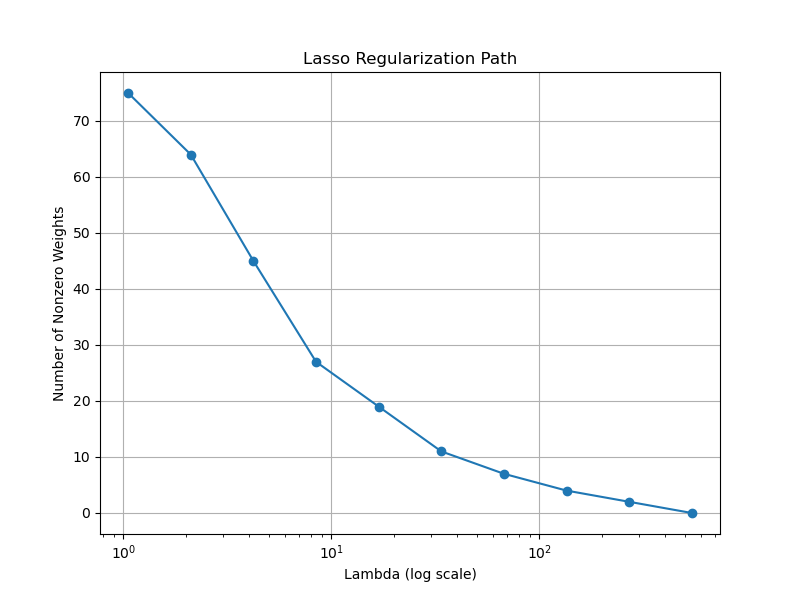
\includegraphics[width=0.8\linewidth]{C:/Users/admin/Downloads/ML/hw2/hw2/reg_path.png}
    \caption{Lasso Regularization Path: Number of nonzero weights as a function of $\lambda$.}
    \label{fig:lasso-path}
\end{figure}

\newpage
\subsection*{(d)}

\begin{figure}[h]
    \centering
    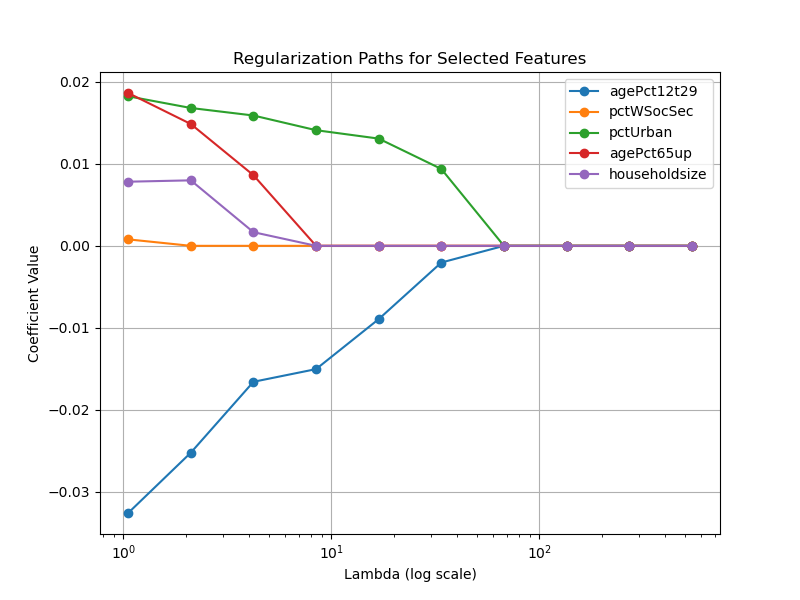
\includegraphics[width=0.8\linewidth]{C:/Users/admin/Downloads/ML/hw2/hw2/reg_path_for_features.png}
    \caption{Regularization Paths for Selected Features: Coefficient values as a function of $\lambda$.}
    \label{fig:feature-paths}
\end{figure}

\newpage
\subsection*{(e)}

\begin{figure}[h]
    \centering
    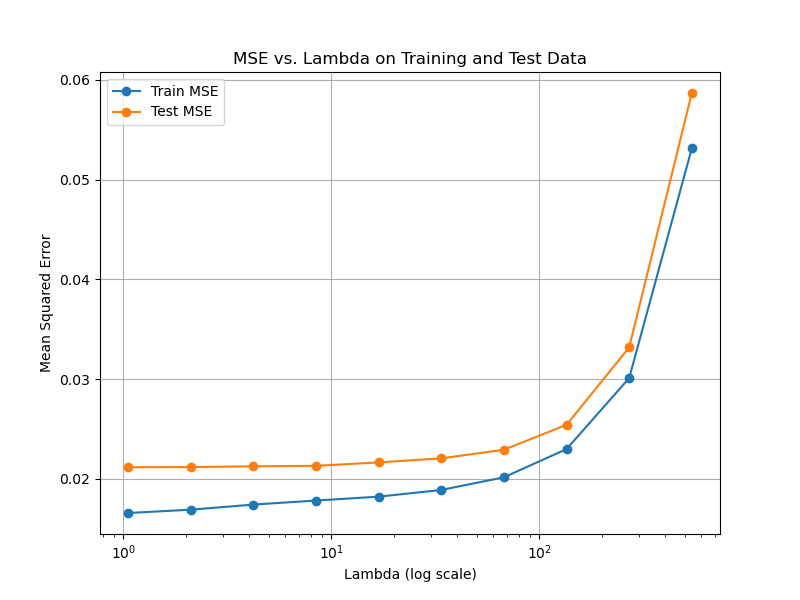
\includegraphics[width=0.8\linewidth]{C:/Users/admin/Downloads/ML/hw2/hw2/mse.png}
    \caption{MSE vs. $\lambda$: Training and test mean squared error as a function of $\lambda$.}
    \label{fig:mse}
\end{figure}

\clearpage  % Forces figures to appear before the code section

\section*{Code Implementation}
\begin{lstlisting}[language=Python]
if __name__ == "__main__":
    from coordinate_descent_algo import train, compute_lambda_max  # type: ignore
else:
    from .coordinate_descent_algo import train

import matplotlib.pyplot as plt
import numpy as np

from utils import load_dataset, problem

def plot_nonzero_weights(lambdas, nonzeros):
    plt.figure(figsize=(8, 6))
    plt.plot(lambdas, nonzeros, marker='o', linestyle='-')
    plt.xscale('log')
    plt.xlabel("Lambda (log scale)")
    plt.ylabel("Number of Nonzero Weights")
    plt.title("Lasso Regularization Path")
    plt.grid(True)
    plt.show(block=False)


def plot_regularization_paths(lambdas, coef_paths):
    plt.figure(figsize=(8, 6))
    for feature, path in coef_paths.items():
        plt.plot(lambdas, path, marker='o', linestyle='-', label=feature)

    plt.xscale('log')
    plt.xlabel("Lambda (log scale)")
    plt.ylabel("Coefficient Value")
    plt.title("Regularization Paths for Selected Features")
    plt.legend()
    plt.grid(True)
    plt.show(block=False)

def compute_mse(X, y, weight, bias):
    predictions = X @ weight + bias
    return np.mean((predictions - y) ** 2)

def plot_mse_vs_lambda(lambdas, mse_train, mse_test):
    plt.figure(figsize=(8, 6))
    plt.plot(lambdas, mse_train, marker='o', linestyle='-', label="Train MSE")
    plt.plot(lambdas, mse_test, marker='o', linestyle='-', label="Test MSE")

    plt.xscale('log')
    plt.xlabel("Lambda (log scale)")
    plt.ylabel("Mean Squared Error")
    plt.title("MSE vs. Lambda on Training and Test Data")
    plt.legend()
    plt.grid(True)
    plt.show()

def train_and_analyze_lasso(X_train, y_train, X_test, y_test, df_train):
    lambda_max = compute_lambda_max(X_train, y_train)
    num_lambdas = 10
    lambdas = [lambda_max / (2**i) for i in range(num_lambdas)]

    nonzeros = []
    mse_train = []
    mse_test = []
    selected_features = ["agePct12t29", "pctWSocSec", "pctUrban", "agePct65up", "householdsize"]
    coef_paths = {feature: [] for feature in selected_features}

    weight = np.zeros(X_train.shape[1])
    for _lambda in lambdas:
        weight, bias = train(X_train, y_train, _lambda, start_weight=weight)

        nonzeros.append(np.count_nonzero(weight))
        mse_train.append(compute_mse(X_train, y_train, weight, bias))
        mse_test.append(compute_mse(X_test, y_test, weight, bias))

        for feature in selected_features:
            coef_paths[feature].append(weight[df_train.columns[1:].tolist().index(feature)])

    plot_nonzero_weights(lambdas, nonzeros)
    plot_regularization_paths(lambdas, coef_paths)
    plot_mse_vs_lambda(lambdas, mse_train, mse_test)

def analyze_largest_coefficients(X_train, y_train, df_train, lambda_value=30):
    weight, _ = train(X_train, y_train, _lambda=lambda_value)
    
    feature_names = df_train.columns[1:].tolist()
    max_feature = feature_names[np.argmax(weight)]
    min_feature = feature_names[np.argmin(weight)]
    
    print(f"Largest positive coefficient feature: {max_feature}")
    print(f"Largest negative coefficient feature: {min_feature}")


@problem.tag("hw2-A", start_line=3)
def main():
    df_train, df_test = load_dataset("crime")

    X_train, y_train = df_train.iloc[:, 1:].values, df_train.iloc[:, 0].values
    X_test, y_test = df_test.iloc[:, 1:].values, df_test.iloc[:, 0].values

    X_mean = np.mean(X_train, axis=0)
    X_std = np.std(X_train, axis=0)
    X_train = (X_train - X_mean) / X_std
    X_test = (X_test - X_mean) / X_std  

    train_and_analyze_lasso(X_train, y_train, X_test, y_test, df_train)
    analyze_largest_coefficients(X_train, y_train, df_train, lambda_value=30)


if __name__ == "__main__":
    main()

\end{lstlisting}

\end{document}
